
\section{Flux optimization}
\subsection{Light flux propagation}

Taking a different approach, we now propose an extended algorithm that
allows to significantly improve the initial design resulting from the
optimized mapping derived in the previous section and allows to design
multiple optical surfaces.  Assuming as in the previous section that
the optical surface is represented as a three-dimensional triangular
mesh, each node of the mesh constituting the first surface has its
position determined by the direction of a source ray (a unit vector),
multiplied by a scalar value. Those directions are held constant
during the construction of the surfaces (only the scalar factors are
varied).

\begin{figure}[!htbp]
  \centering 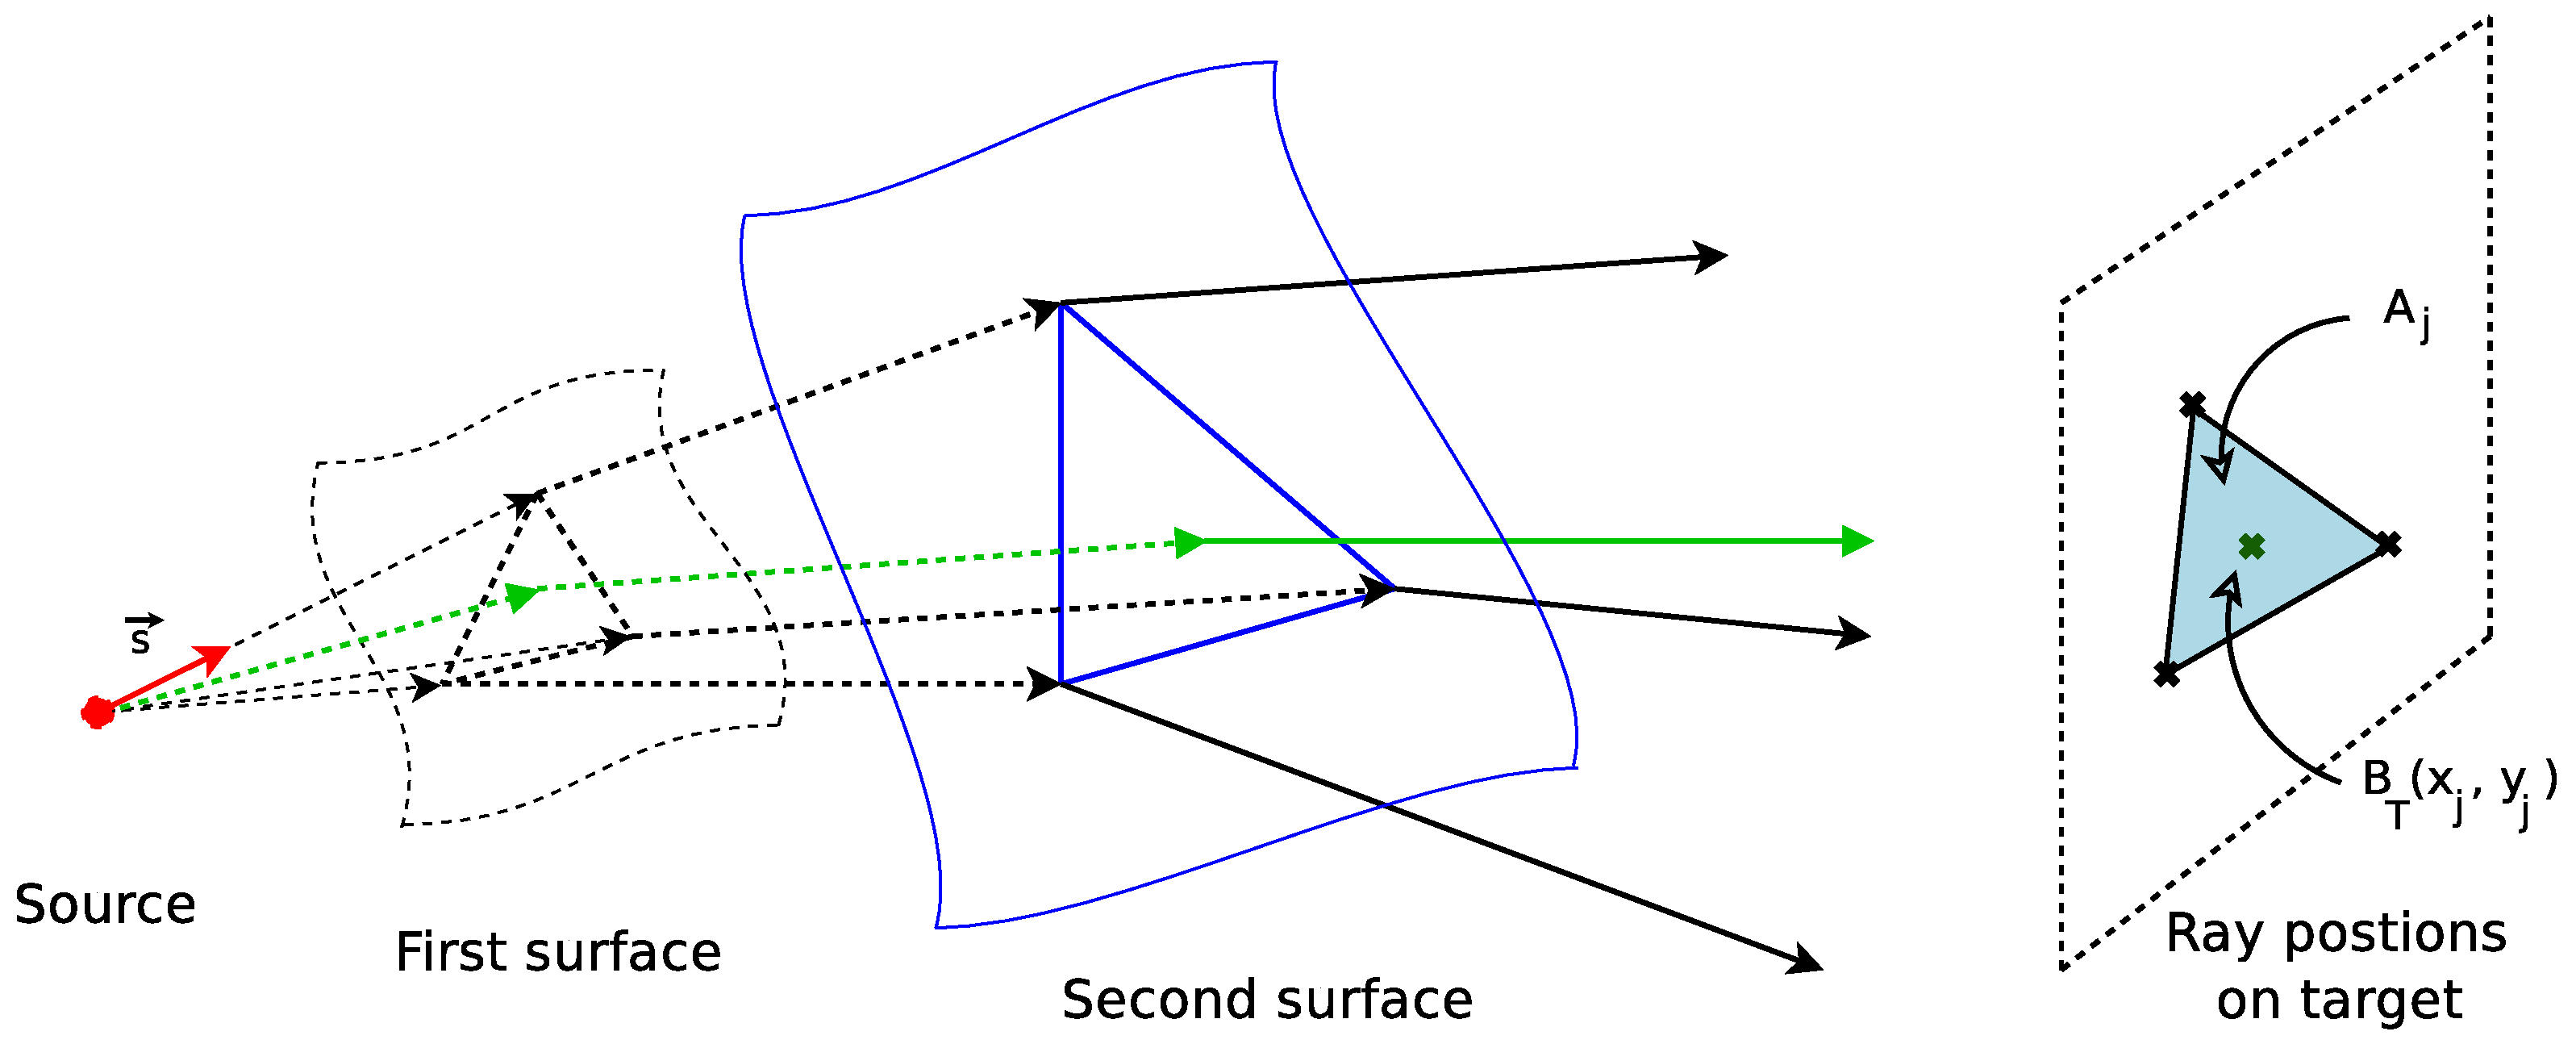
\includegraphics[width=0.9\textwidth]{rays_new}
  \caption{Elementary light flux tube (prism-shaped) delimited by the rays passing
    through the vertices of a triangular surface element (blue). The
    vertex rays are represented in dark, the face ray in green.  If
    the vertex ray \textit{directions} (e.g. the red vector
    $\mathbf{s}$) drawn from the source are held constant, the light
    flux within the triangular tube also remains constant.}
  \label{fig:rays}
\end{figure}


We observe that, on the one hand, the flux emitted by the source
$\Phi_S$ can be written as follows:
\begin{itemize}
\item for a point source:
  \begin{equation}
   \Phi_S = \iint d^2\Phi_S = \iint I(\theta, \phi) d^2\Omega
   \label{eq:flux_src_point}
  \end{equation}
  where $d^2\Phi_S$ is the elementary light flux, $d^2\Omega$ the
  elementary solid angle surrounding the direction of emission
  $(\theta, \phi)$, and $I(\theta, \phi)$ is the radiant intensity (in
  $\mathrm{W/sr}$) of the point source.  The elementary solid angle
  $d^2\Omega$ is approximated by the solid angle encompassed by the
  three source rays around a triangular face
  (see~Fig.~\ref{fig:rays}).  This solid angle remains constant
  throughout the construction.

\item for a collimated source:
  \begin{equation}
   \Phi_S = \iint d^2\Phi_S = \iint B_S(x, y) dx\,dy 
   \label{eq:flux_src_coll}
  \end{equation}
  where $B_S(x,y)$ is the source (radiant) irradiance (in $\mathrm{W/m^2}$).  In
  this case, the source rays are all directed towards the
  same direction (e.g. along the $z$-axis) and the cross section of a
  triangular tube remains constant between the source and the first
  optical surface.
\end{itemize}
In both cases, the flux from the source within a triangular tube
remains constant along its path through the optical system,
 as illustrated by Fig.~\ref{fig:rays}.

On the other hand, the flux reaching the target $\Phi_T$ can be
written as a function of the irradiance (in $\mathrm{W/m^2}$) on the target.  A
triangular flux tube is projected as a triangular area on the target
as illustrated in Fig.~\ref{fig:rays}.  The flux in this tube can be
computed as:
\[ \Phi_T(j) = \iint_{A_j} B_T(x, y) dx\,dy \]
where $A_j$ is the area of the target triangle corresponding to the
$j$-th face of the surface, and $B_T(x,y)$ the desired irradiance at
the target point $(x,y)$. This integral is approximated with the
simplest quadrature:
\begin{equation}
  \Phi_T(j) = B_T(x_j, y_j) A_j
  \label{eq:flux_target}
\end{equation}  
with $(x_j, y_j)$ being the center of the triangular face on the
target as illustrated in~Fig.~\ref{fig:rays}.


\subsection{Smoothing terms}

\subsubsection{Objective function components}
Similarly to the purely mapping-based approach in~\cite{Baeuerle2012},
a least-squares optimization procedure is proposed. Taking into
account the description of the light flux above, the merit function
being optimized can now be detailed as a collection of three
components:

\begin{itemize}
\item{\emph{light flux difference}}: this component aims to equalize
  the light flux in Eqs.~\eqref{eq:flux_src_point} (or
  \eqref{eq:flux_src_coll}) and~\eqref{eq:flux_target}. It ensures
  that the desired irradiance $B_T(x, y)$ is achieved on the target;
\item{\emph{smoothing component}}: in order to avoid local minima
  corresponding to triangular mesh components with abnormally high or
  low radiant intensity values (distorted triangles), a smoothing component is
  added. It enforces that face rays intersect the target near the
  center of the respective triangular area on the target. 
  A face ray is closely correlated to the normal vector of the 
  corresponding triangular face on the optical surface. Thus this 
  component gives the advantage to nearly co-planar neighbor triangles 
  on the optical surface;
\item{\emph{distance to target's boundary}}: the source and the target
  total light flux are both normalized to unity, so that all the
  source rays going through the system must eventually reach the
  target. This is explicitly enforced by penalizing edge rays which
  deviate too far from the target boundary.
\end{itemize}

\subsubsection{Numerical considerations}
A consistent and homogeneous scaling of the three merit function
components allows a better numerical stability, the ability to easily
scale up or down the resolution of the surface (number of triangles),
or the possibility to change the geometry of the problem without
re-adjusting from scratch the convergence criteria of the optimizer.

All three components of the objective function above are hence chosen
to be homogeneous to unity and to remain of the same order of
magnitude, regardless of the geometry or resolution of the problem:
\begin{itemize}
\item the flux difference for a face is multiplied by the number of
  faces.  Since the source flux is already normalized to unity, this
  ensures the scalability with regards to the number of triangles in
  the mesh. The effective light flux going through a face hence always
  has the order of magnitude unity;
\item the smoothing component is scaled by the typical size of a
  triangle area on the target which varies as the square root of the
  total number of triangles;
\item the distance to the target boundary is scaled by the target
  size.
\end{itemize}

The optimization procedure also involves the computation of a
numerical gradient in the form of a standard forward difference using
a step size $h$. It can be shown\cite{Bindel2009} that on a
finite-precision machine with machine precision $\epsilon_m$ such a
computation leads to the following final relative error:
\begin{equation}
 \tilde{f'}(x) = f'(x) \left(1 + \epsilon_m \frac{2f(x)}{hf'(x)} +
 \frac{f''(x)}{2f'(x)}h \right)
 \label{eq:grad_error}
\end{equation}
with $\tilde{f'}(x)$ the numerical approximation of the derivative and
$\epsilon_m$ the machine round-off precision.  The last two terms are
competing one with another and dictate an optimal value for $h$.
Noting $\epsilon_m = 10^m$, $h = 10^n$, ${2f}/(hf') = 10^u$ and
${f''(x)}/(2f'(x)) = 10^v$ the optimal value of $n$ satisfies $ v+n =
-n+u+m $, hence:
\[n = (u-v+m)/2\]
Typically, with the scaling considerations mentioned above $(u,v,m) =
(-1, -1, -15)$ giving a step size $h \approx 10^{-7}$ and an overall
relative computation precision around $\epsilon = 10^{v+n} \approx
10^{-8}$.  However the computation above discards the error induced by
the evaluation of $f$ itself (propagation error): a slightly bigger
step size (around $h \approx 10^{-6}$) gives in practice better
results and has been retained in the final implementation.

Finally, the computation time using this new objective function is
about a factor 4 longer than the mapping-only approach, but this remains 
within minutes on a standard PC for typical applications (general lighting,
automotive, etc ...).

\section{Sample applications}
\label{sec:results}
The procedure presented above allows the design of various optical
configurations with a wide range of applications. We present two
complex cases. For each design below the improvement between the
initial mapping approach and the flux optimized approach is presented,
and the examples are given in order of increasing difficulty.

\subsection{Double sided freeform lens}
First, a refractive case with two freeform surfaces is presented.  The
target plane is positioned perpendicular to the light axis and is
centered on it at a distance of $100\mathrm{~mm}$.  The prescribed irradiance
is the letter~``B''.

\begin{figure}[!htbp]
  \centering \includegraphics[width=1.0\textwidth]{app-B}
  \caption{Double sided freeform lens projecting the letter ``B''
    (lengths in~$\rm mm$, irradiance in~$\rm a.u.$); (a) with mapping
    optimization only; (b) with mapping and flux optimization; (c)
    lens CAD model, the source is positioned at the origin of the
    coordinate system.  }
  \label{fig:letter}
\end{figure}

The flux optimization provides a sharper cut-off at the boundaries of
the pattern as can be seen in the two middle holes, and on the upper
and lower tips of the left part of the distribution.  The two freeform
surfaces forming the lens were designed using 4,000 triangles for each
optical element.  The final surfaces consist of two NURBS fitted to
the two triangular meshes.  The design assumes that the lens is made
of glass ($n=1.5$) and that a light cone with a half-angle of
45~degrees is captured from the point source.
%%% CONFLICTING with what Loo said, but I prefer Reviewer 1's comment:
%The resulting optical efficiency amounts to 46\%
%(including Fresnel losses).

\subsection{Logo lens}
To demonstrate the abilities of the presented algorithm a much more
elaborate example is presented.  The optics has been designed for a
perfectly collimated source. The logo is projected on a surface of $55
\times 17.5\,mm^2$ at a distance of $100\,mm$ from the source, and has
a resolution of $530 \times 160$~pixels. We present the results with
one and two freeform surfaces, respectively. The optics has a size
close to the target one: $50 \times 15\,mm^2$.

\begin{figure}[!htbp]
  \centering 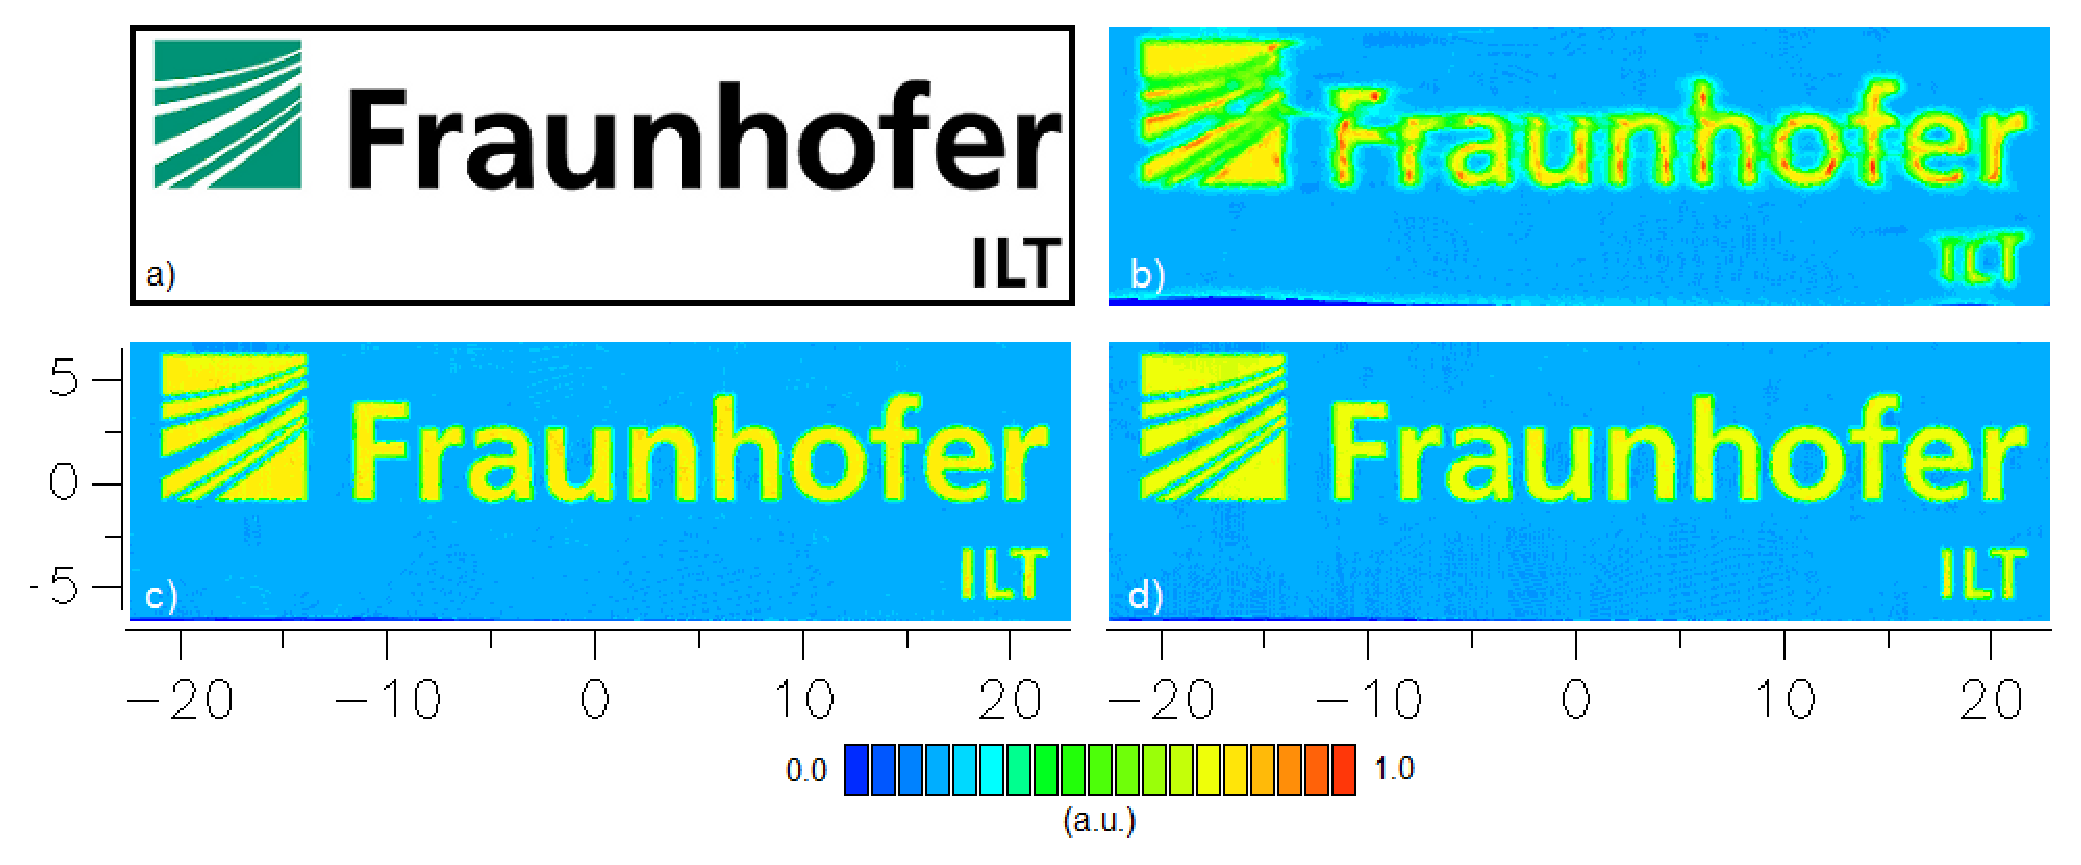
\includegraphics[width=1.0\textwidth]{logo_bottom}
  \caption{Ray-tracing of high-resolution logo generated with 16
    million rays (lengths in~$\rm mm$, irradiance in~$\rm a.u.$); (a)
    prescribed irradiance distribution (passed to the algorithm in
    black and white); (b) one freeform surface with mapping
    optimization only; (c) one freeform surface with mapping and flux
    optimization; (d) two freeform surfaces with mapping and flux
    optimization.}
  
  \label{fig:logo}
\end{figure}

The ray tracings presented in Fig.~\ref{fig:logo} were performed with
16~million rays and a detector grid having the same resolution as the
prescribed irradiance.  Once again, the improvement over the mapping
optimization is clearly visible: the contours of the letters making
the logo are much sharper and better defined, particularly in the
bottom right part (see analysis focused on the ``ILT'' part
below). The overall result looks equally satisfactory with one or two
freeform surfaces.

Similar to what has been done previously by Bortz and
Shatz~\cite{Bortz2007}, the following fractional RMS measure was
computed to assess the quality of the design:
\begin{equation}
  RMS= \sqrt{\sum\left(\frac{I_c - I_p}{I_{ref}}\right)^2}
  \label{eq:rms}
\end{equation} 
where $I_c$ is the computed irradiance as given by the ray tracing,
$I_p$ is the prescribed irradiance and $I_{ref}$ is a reference
irradiance.  Bortz and Shatz restricted their computation to an area
where the irradiance was sufficiently high and hence took
$I_{ref} = I_p$.  In our case, given the contrast at hand (about 4:1)
and the fact that the analysis should not be restrained to the letter
cores (areas of high irradiance), we computed the RMS with both
$I_{ref} = I_{avg}$, the (arithmetical) average of the light
irradiance, and $I_{ref} = I_{max}$, the peak irradiance found at the
core of a letter, for example.

For statistical relevance, the analysis was also restrained on a
sub-part of the logo where a fine level of details is found
(see~Fig.~\ref{fig:logo_zoom}).  The sub-area was traced with
2~million rays and covers $66\times39$~detector pixels.  With this
setup the ray tracing of a homogeneous pattern would result in a
statistical relevance of 3-4\%.

\begin{figure}[!htbp]
  \centering 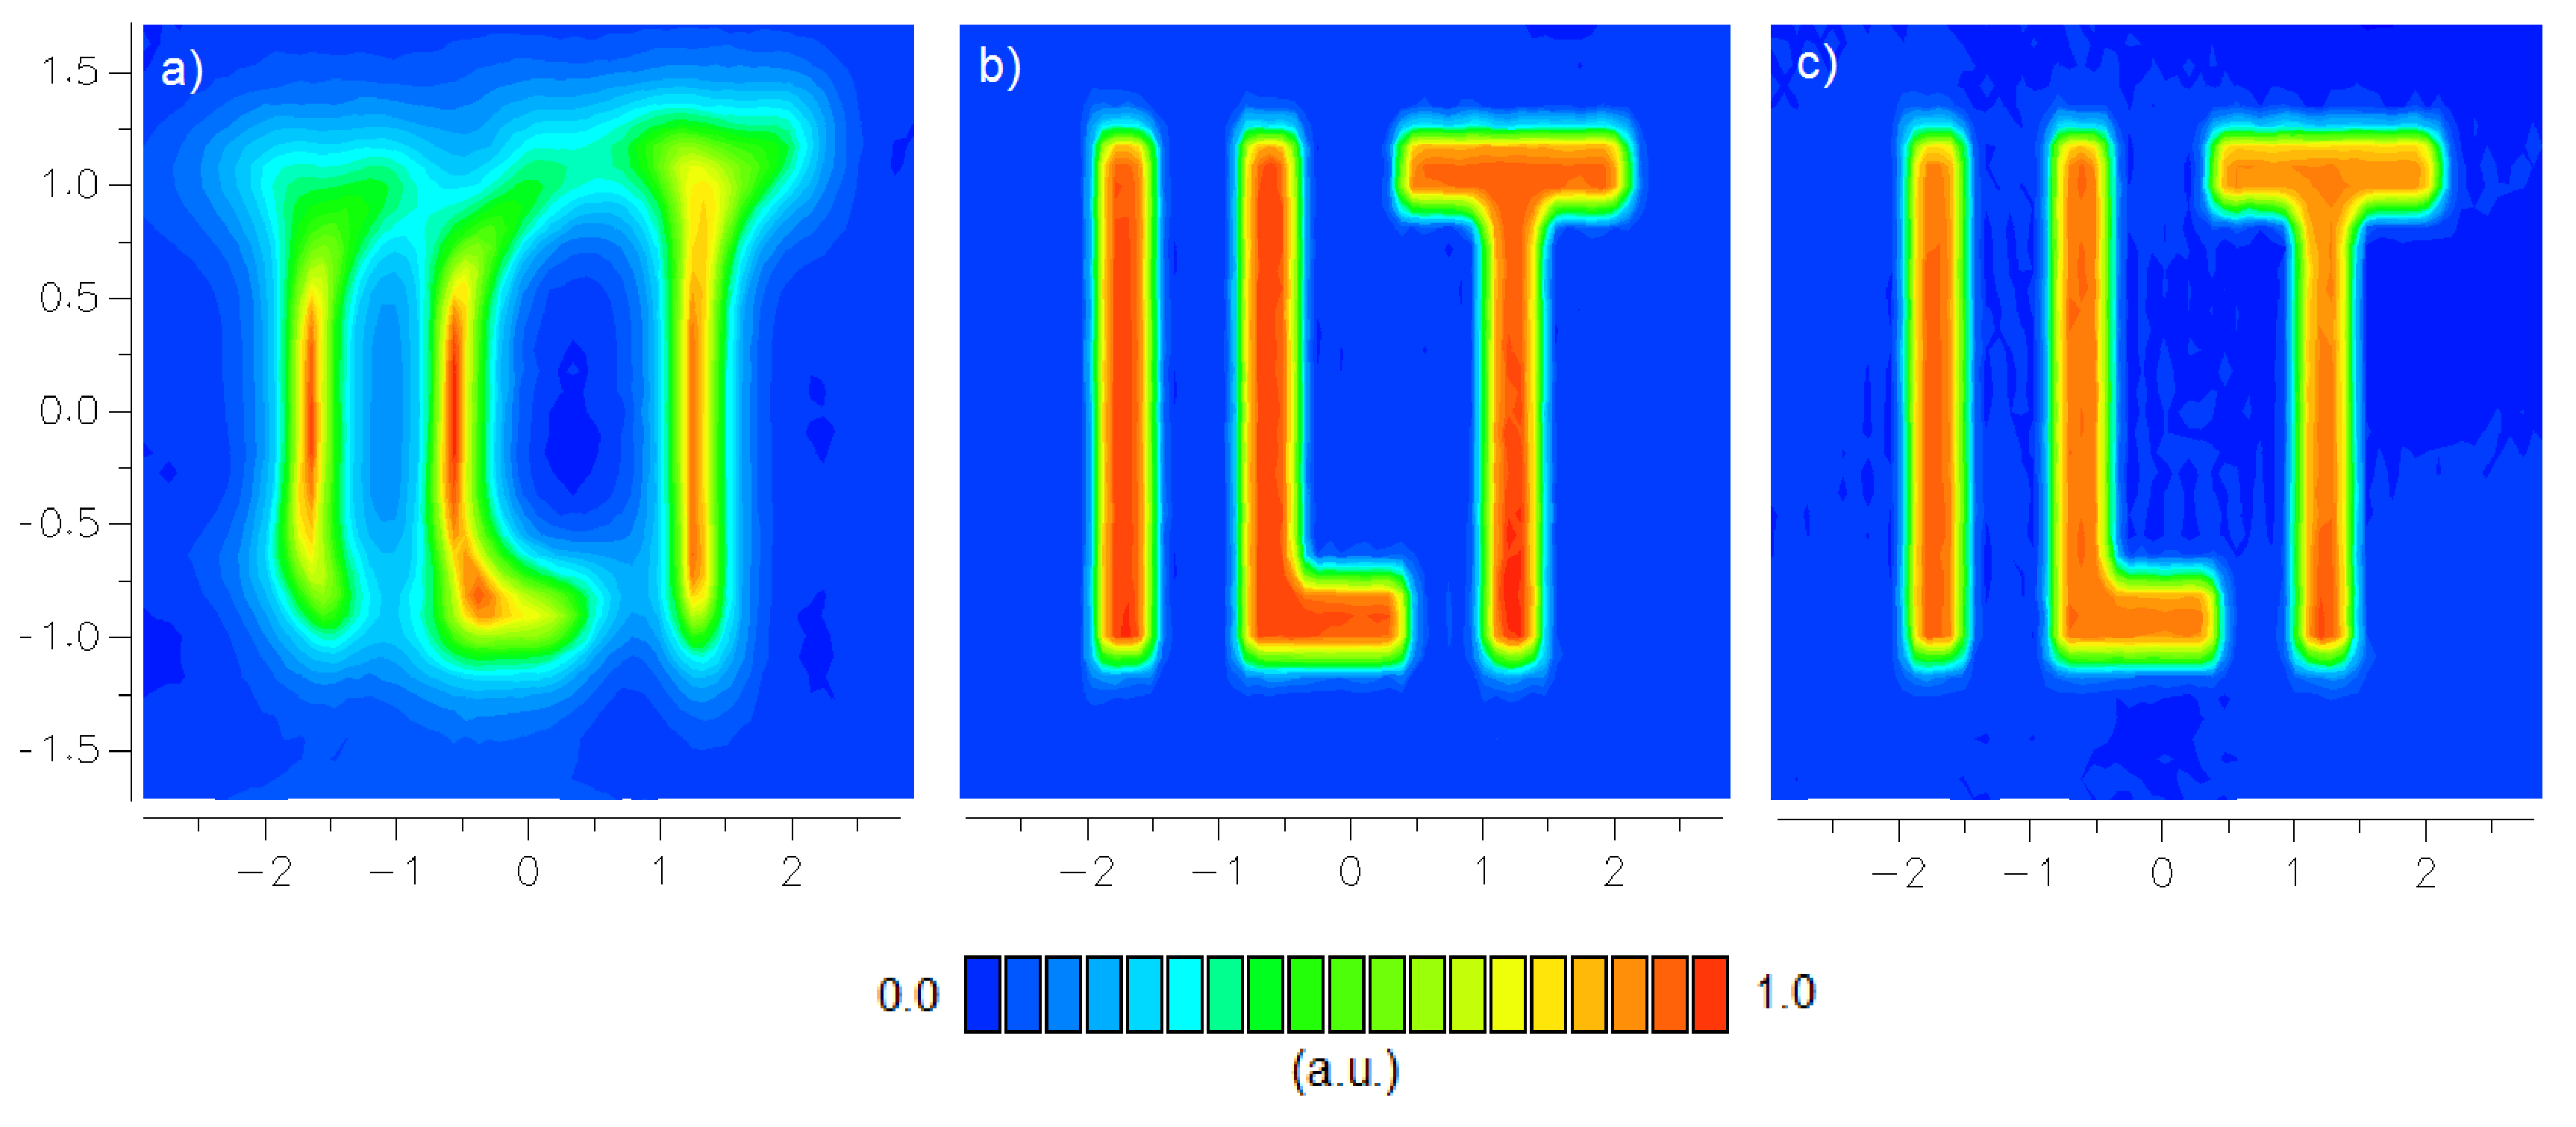
\includegraphics[width=0.95\textwidth]{logo_zoom}
  \caption{Zoom on the lower right part of the logo for RMS
    analysis. Ray-tracing with 2 million rays on a grid of $66 \times 39$
    points (lengths in~$\rm mm$, irradiance in~$\rm a.u.$). 
    (a) one freeform surface with mapping optimization only; 
    (b) one freeform surface with mapping and flux optimization;
    (c) two freeform surfaces with mapping and flux optimization.}
  \label{fig:logo_zoom}
\end{figure}

Table~\ref{tab:rms} presents the resulting fractional RMS computed
with the two different irradiance references (average and maximum).
\begin{table}[!htbp]
  \centering
  \caption{Fractionnal RMS for a sub-area of the logo
    projection. $RMS_{avg}$ (resp. $RMS_{max})$ denotes the RMS
    computed with $I_{ref}$ being the average irradiance (resp. with
    $I_{ref}$ being the peak irradiance)}
  \label{tab:rms}
  \begin{tabular}{c|c|c|}
    \cline{2-3}
      & $RMS_{avg}$ & $RMS_{max}$ \\ \hline
    \multicolumn{1}{|c|}{One surface (mapping optimization only)} 
      & 33.7\% & 16.0\% \\\hline
    \multicolumn{1}{|c|}{One surface (mapping and flux optimization)}
      & 10.1\% & 4.82\% \\\hline 
    \multicolumn{1}{|c|}{Two surfaces (mapping and flux optimization)}
      & 10.2\% & 4.84\% \\\hline
\end{tabular}
\end{table} 
The improvement brought on by the flux optimization is clearly visible for
both references.  The last two lines show that the ray-tracing falls
slightly off the statistical boundary given above. The sharp edges of
the letters forming the logo are challenging to project and prove to
be the main deteriorating factor.  Comparing part b) and c) of
Fig.~\ref{fig:logo_zoom}, we can also identify a slight loss of
irradiance homogeneity within the letters, confirming that the single
surface design is less complicated.  However, in both cases, the shape
of the pattern has clear and well defined contours.

Finally the overall optical efficiency in this case is close to its
maximum theoretical value, since all the rays of the collimated source
are captured by the optical system.

